\documentclass[a4paper,12pt]{article}

% ─── Pacotes ────────────────────────────────────────────────────────────────
\usepackage[T1]{fontenc}
\usepackage[utf8]{inputenc}
\usepackage[brazil]{babel}
\usepackage[margin=2cm]{geometry}
\usepackage{graphicx}
\usepackage{booktabs}
\usepackage{xcolor}
\usepackage{colortbl}
\usepackage{array}
\usepackage{caption}
\usepackage{subcaption}
\usepackage{hyperref}
\usepackage{fancyhdr}
\usepackage{mdframed}
\usepackage{enumitem}
\usepackage{amssymb}

% ─── Caminhos de imagem ─────────────────────────────────────────────────────
\graphicspath{{../../images/}}

% ─── Cabeçalho / Rodapé ─────────────────────────────────────────────────────
\pagestyle{fancy}
\fancyhf{}
\lhead{\textbf{Revisão de Figuras — IEEE Access}}
\rhead{\textit{Context-oriented Synthesis of Salt Domes}}
\cfoot{\thepage}

% ─── Cores de status ────────────────────────────────────────────────────────
\definecolor{ok}{RGB}{200,240,200}
\definecolor{atencao}{RGB}{255,243,180}
\definecolor{problema}{RGB}{255,200,200}
\definecolor{unused}{RGB}{220,220,220}

% ─── Ambiente checkblock ────────────────────────────────────────────────────
\newmdenv[
  linecolor=gray!50,
  backgroundcolor=gray!5,
  roundcorner=4pt,
  innertopmargin=6pt,
  innerbottommargin=6pt,
]{checkblock}

% ─── Ambiente quoteblock ────────────────────────────────────────────────────
\newmdenv[
  linecolor=blue!30,
  backgroundcolor=blue!4,
  roundcorner=4pt,
  innertopmargin=6pt,
  innerbottommargin=6pt,
]{quoteblock}

% ─── Comando \figentry{número}{arquivo}{label}{status} ──────────────────────
\newcommand{\figentry}[4]{%
  \subsection*{Figura~#1 \quad \texttt{#2}}
  \noindent\textbf{Label:} \texttt{#3}\hfill\textbf{Status:} #4\\[4pt]
}

% ────────────────────────────────────────────────────────────────────────────
\begin{document}

\begin{center}
  {\LARGE\bfseries Revisão de Figuras do Manuscrito}\\[6pt]
  {\large IEEE Access — \textit{Context-oriented Synthesis of Salt Domes}}\\[4pt]
  {\large Luciano D.\ Terres \& Jacob Scharcanski}\\[2pt]
  {\normalsize Data de revisão: \today}
\end{center}
\vspace{0.5cm}
\hrule
\vspace{0.5cm}

% ─── Tabela-resumo ───────────────────────────────────────────────────────────
\section*{Tabela-Resumo}

\begin{table}[h!]
\centering
\caption*{\textbf{Status de cada figura}}
\renewcommand{\arraystretch}{1.4}
\begin{tabular}{clllc}
\toprule
\textbf{Fig.} & \textbf{Arquivo} & \textbf{Uso no manuscrito} & \textbf{Status} & \textbf{Ação?} \\
\midrule
\rowcolor{ok}      1  & terre1.png  & Fig.\ 1 --- Pipeline            & OK         & \\
\rowcolor{ok}      2  & terre2.png  & Fig.\ 2 --- VAE Masks           & OK         & \\
\rowcolor{ok}      3  & terre3.png  & Fig.\ 3 --- Edge/Boundary       & OK         & \\
\rowcolor{ok}      4  & terre4.png  & Fig.\ 4 --- Border zones        & OK         & \\
\rowcolor{ok}      5  & terre5.jpg  & Fig.\ 5 --- Texture synthesis   & OK         & \\
\rowcolor{ok}      6  & terre6.png  & Fig.\ 6 --- Context zones       & OK         & \\
\rowcolor{unused}  7  & terre7.png  & Nao usada no \_v7.tex atual     & NAO USADA  & Verificar \\
\rowcolor{unused}  8  & terre8.png  & Sem referencia encontrada       & NAO USADA  & Verificar \\
\rowcolor{ok}      9  & terre9.png  & Synthetic Samples               & OK         & \\
\rowcolor{ok}     10  & terre10.png & Quantitative analysis           & OK         & \\
\rowcolor{unused} 11  & terre11.png & Sem referencia encontrada       & NAO USADA  & Verificar \\
\rowcolor{ok}     B1  & terre.jpg   & Foto --- Luciano D.\ Terres     & OK         & \\
\rowcolor{ok}     B2  & schar.jpg   & Foto --- Jacob Scharcanski      & OK         & \\
\bottomrule
\end{tabular}
\end{table}

\bigskip
\noindent\textbf{Legenda de cores:}
\quad \colorbox{ok}{\strut~OK~}
\quad \colorbox{atencao}{\strut~Atencao~}
\quad \colorbox{problema}{\strut~Problema~}
\quad \colorbox{unused}{\strut~Nao usada~}

\newpage

% ════════════════════════════════════════════════════════════════════════════
\section*{Revisao Individual das Figuras}
% ════════════════════════════════════════════════════════════════════════════

% ─── Figura 1 ────────────────────────────────────────────────────────────────
\figentry{1}{terre1.png}{fig:synthesis\_pipeline}{\colorbox{ok}{OK}}

\begin{figure}[h!]
  \centering
  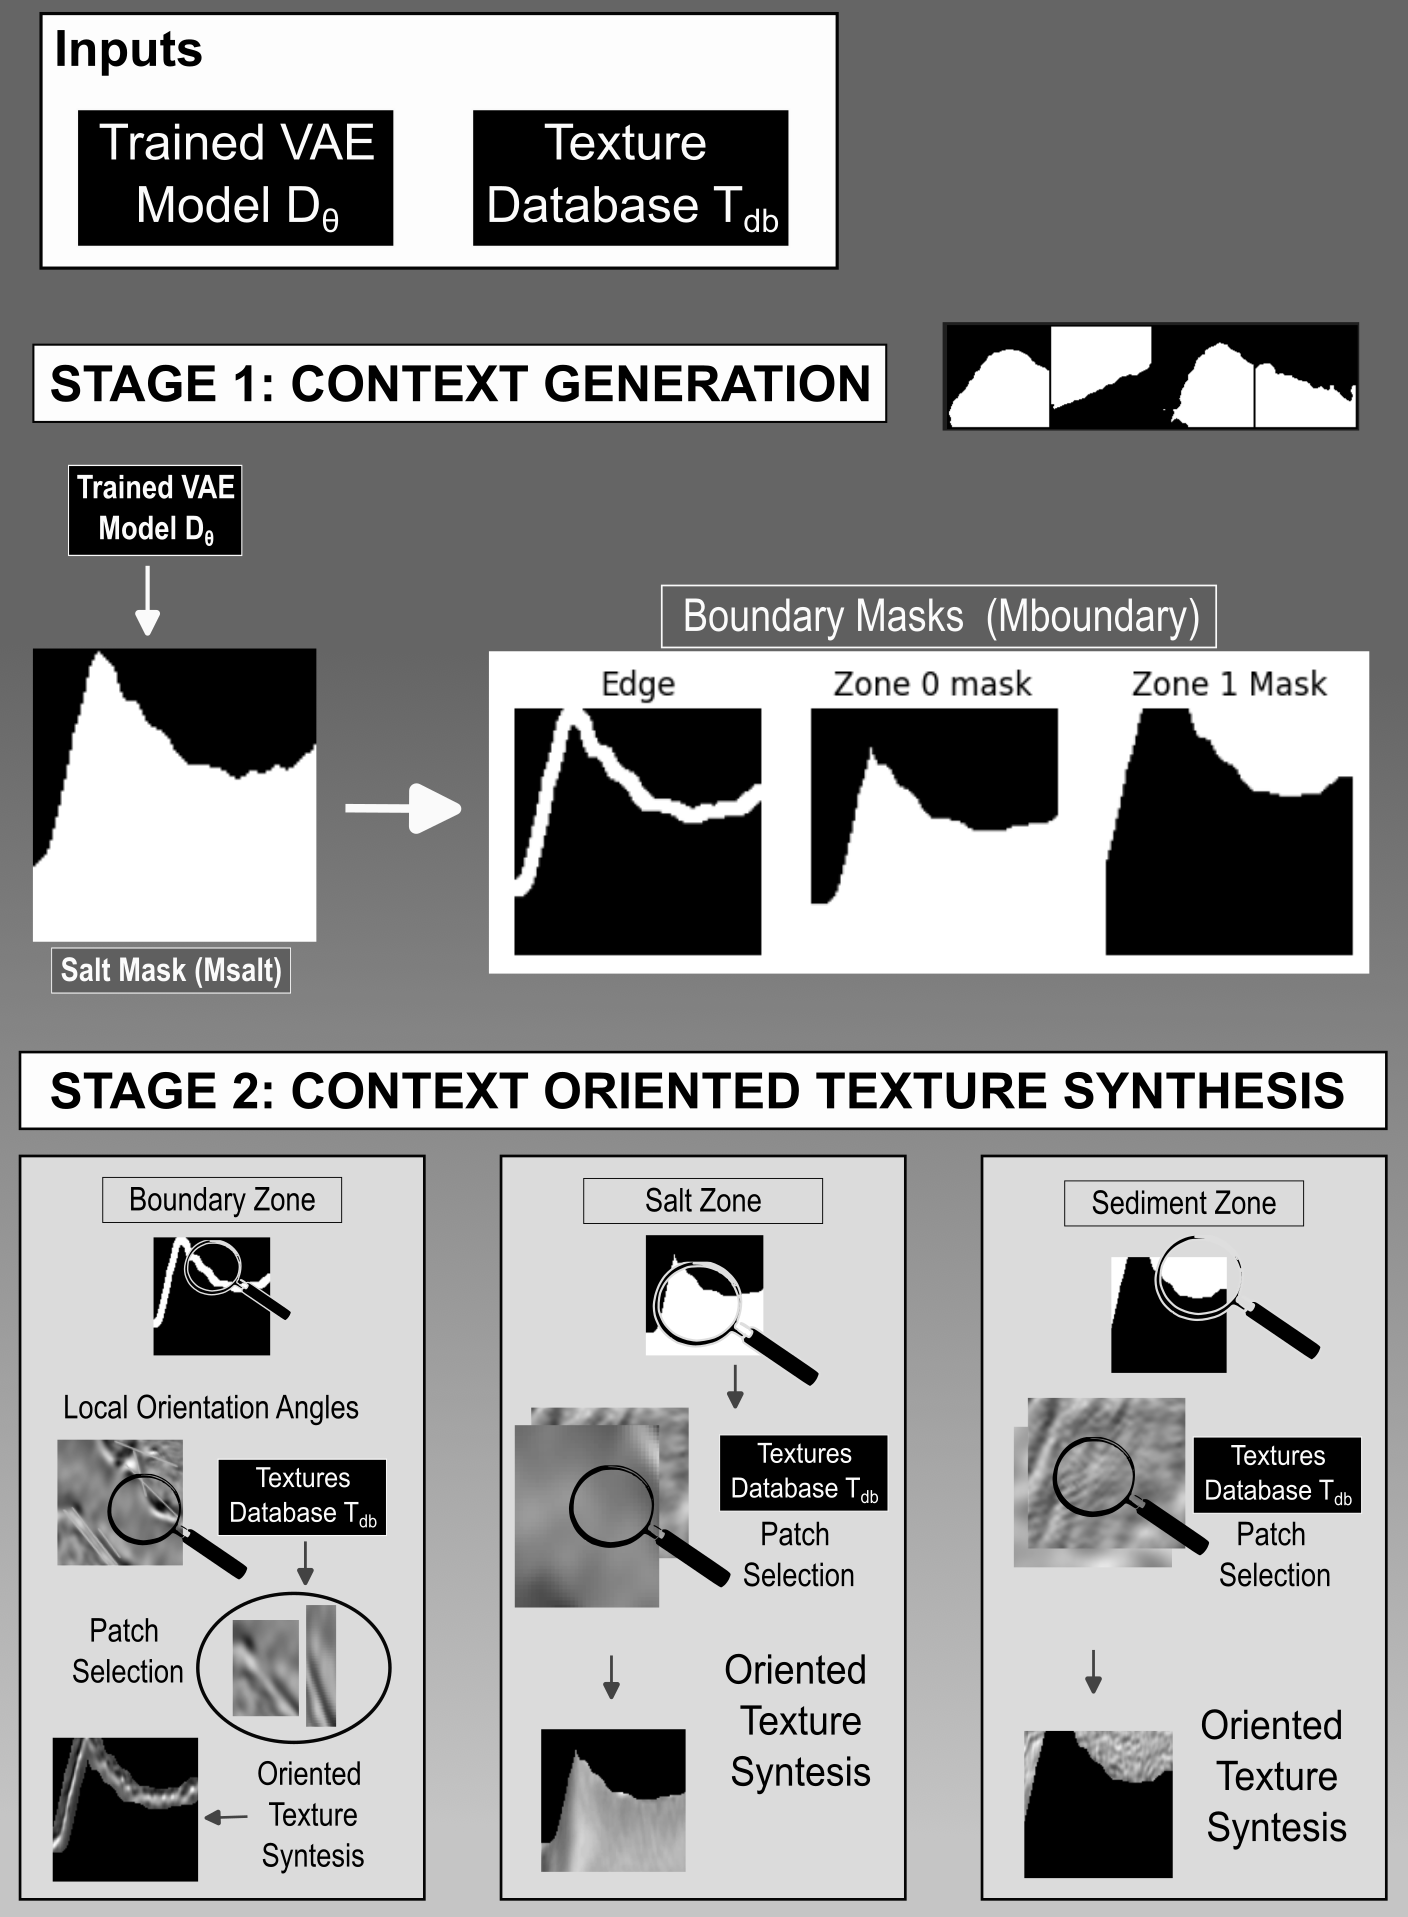
\includegraphics[width=0.7\linewidth]{terre1.png}
  \caption*{\textbf{Legenda:} \textit{``Complete pipeline of the proposed context-oriented seismic image synthesis methodology, showing the integration of VAE-based mask generation and the context-aware texture synthesis method.''}}
\end{figure}

\noindent\textbf{Citacao no manuscrito \texttt{(\_v7.tex, l.\,109)}:}
\begin{quoteblock}
\small
``[\ldots] The proposed method focuses on context zones and on the characteristics of seismic
images with salt domes, ensuring that the synthetic samples preserve the structural and
textural properties of real seismic imaging data. \textbf{Figure~1 illustrates the complete synthesis
pipeline}, showing how the VAE-generated masks are combined with context-oriented texture
synthesis to produce realistic synthetic seismic images.''
\end{quoteblock}

\begin{checkblock}
\textbf{Checklist IEEE Access:}
\begin{itemize}[leftmargin=1.5em,topsep=2pt,itemsep=1pt]
  \item[$\square$] Resolucao $\geq$ 300 DPI (fotografias) / $\geq$ 600 DPI (line art)
  \item[$\square$] Sem fundo cinza / sem artefatos de captura de tela
  \item[$\square$] Texto legivel apos reducao para coluna simples ($\approx$ 8,5 cm)
  \item[$\square$] Exportado diretamente do programa-fonte (nao screenshot)
  \item[$\square$] Cores funcionam em escala de cinza
\end{itemize}
\end{checkblock}

\noindent\textbf{Notas de revisao:}
\begin{mdframed}[linecolor=gray!30,backgroundcolor=white,innertopmargin=8pt,innerbottommargin=8pt]
  \vspace{3cm}
\end{mdframed}

\newpage

% ─── Figura 2 ────────────────────────────────────────────────────────────────
\figentry{2}{terre2.png}{fig:vae1}{\colorbox{ok}{OK}}

\begin{figure}[h!]
  \centering
  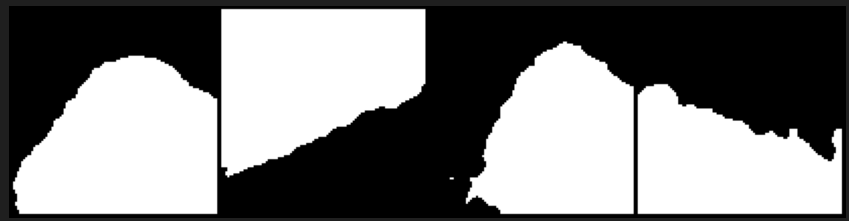
\includegraphics[width=0.7\linewidth]{terre2.png}
  \caption*{\textbf{Legenda:} \textit{``Samples of generated structural salt masks. The Variational Autoencoder learns the features distribution and produces new structural masks.''}}
\end{figure}

\noindent\textbf{Citacao no manuscrito \texttt{(\_v7.tex, l.\,121 e l.\,131)}:}
\begin{quoteblock}
\small
(1)~``The proposed data augmentation scheme detects and generates new rock geometries with a
VAE, \textbf{as illustrated in Fig.~2}.''\\[4pt]
(2)~``\textbf{Fig.~2 illustrates a dataset of seismic images} used to generate new salt dome masks.
The natural intersection between two different rocks are their boundaries, and in the case of
salt rocks, this boundary usually is apparent, as Fig.~3 shows.''
\end{quoteblock}

\begin{checkblock}
\textbf{Checklist IEEE Access:}
\begin{itemize}[leftmargin=1.5em,topsep=2pt,itemsep=1pt]
  \item[$\square$] Resolucao $\geq$ 300 DPI
  \item[$\square$] Sem fundo cinza / sem artefatos
  \item[$\square$] Texto legivel na largura de coluna
  \item[$\square$] Exportado diretamente do programa-fonte
  \item[$\square$] Cores funcionam em escala de cinza
\end{itemize}
\end{checkblock}

\noindent\textbf{Notas de revisao:}
\begin{mdframed}[linecolor=gray!30,backgroundcolor=white,innertopmargin=8pt,innerbottommargin=8pt]
  \vspace{3cm}
\end{mdframed}

\newpage

% ─── Figura 3 ────────────────────────────────────────────────────────────────
\figentry{3}{terre3.png}{fig:edge1}{\colorbox{ok}{OK}}

\begin{figure}[h!]
  \centering
  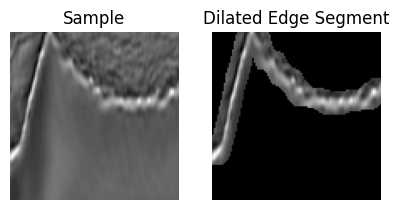
\includegraphics[width=0.7\linewidth]{terre3.png}
  \caption*{\textbf{Legenda:} \textit{``Sample of the boundaries identification between salt and other sediments represented in a dilated edge segment.''}}
\end{figure}

\noindent\textbf{Citacao no manuscrito \texttt{(\_v7.tex, l.\,131 e l.\,280)}:}
\begin{quoteblock}
\small
(1)~``[\ldots] in the case of salt rocks, this boundary usually is apparent,
\textbf{as Fig.~3 shows}. During the VAE training process, we use only salt masks with a
considerable amount of salt, varying from 10 to 90 percent of the total area.''\\[4pt]
(2)~``[\ldots] a boundary strip of 5 pixels total width. \textbf{As Fig.~3 shows}, this strip is an
area of high seismic contrast appearing as light and dark bands.''
\end{quoteblock}

\begin{checkblock}
\textbf{Checklist IEEE Access:}
\begin{itemize}[leftmargin=1.5em,topsep=2pt,itemsep=1pt]
  \item[$\square$] Resolucao $\geq$ 300 DPI
  \item[$\square$] Sem fundo cinza / sem artefatos
  \item[$\square$] Texto legivel na largura de coluna
  \item[$\square$] Exportado diretamente do programa-fonte
  \item[$\square$] Cores funcionam em escala de cinza
\end{itemize}
\end{checkblock}

\noindent\textbf{Notas de revisao:}
\begin{mdframed}[linecolor=gray!30,backgroundcolor=white,innertopmargin=8pt,innerbottommargin=8pt]
  \vspace{3cm}
\end{mdframed}

\newpage

% ─── Figura 4 ────────────────────────────────────────────────────────────────
\figentry{4}{terre4.png}{fig:line1}{\colorbox{ok}{OK}}

\begin{figure}[h!]
  \centering
  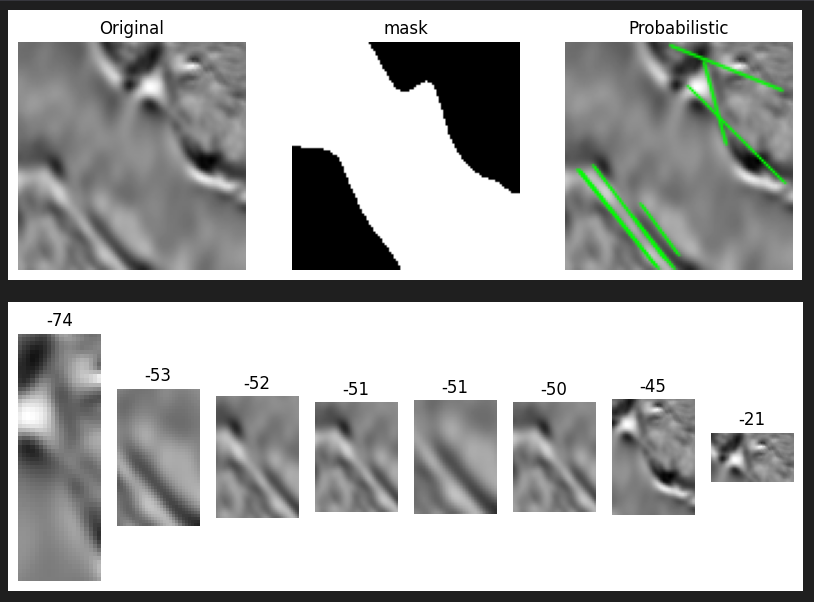
\includegraphics[width=0.7\linewidth]{terre4.png}
  \caption*{\textbf{Legenda:} \textit{``The green lines at original image identify border zones and angles to guide the patch selection in the patch database construction process.''}}
\end{figure}

\noindent\textbf{Citacao no manuscrito \texttt{(\_v7.tex, l.\,280)}:}
\begin{quoteblock}
\small
``[\ldots] As Fig.~3 shows, this strip is an area of high seismic contrast appearing as light and
dark bands. Also, various parallel lines make up this boundary, and \textbf{Fig.~4 shows their angles}.
We use a dataset composed of edge pieces and their corresponding angles as input for the
boundary synthesis process.''
\end{quoteblock}

\begin{checkblock}
\textbf{Checklist IEEE Access:}
\begin{itemize}[leftmargin=1.5em,topsep=2pt,itemsep=1pt]
  \item[$\square$] Resolucao $\geq$ 300 DPI
  \item[$\square$] Sem fundo cinza / sem artefatos
  \item[$\square$] Linhas verdes visiveis e nitidas
  \item[$\square$] Exportado diretamente do programa-fonte
  \item[$\square$] Cores funcionam em escala de cinza
\end{itemize}
\end{checkblock}

\noindent\textbf{Notas de revisao:}
\begin{mdframed}[linecolor=gray!30,backgroundcolor=white,innertopmargin=8pt,innerbottommargin=8pt]
  \vspace{3cm}
\end{mdframed}

\newpage

% ─── Figura 5 ────────────────────────────────────────────────────────────────
\figentry{5}{terre5.jpg}{fig:edge2}{\colorbox{ok}{OK}}

\begin{figure}[h!]
  \centering
  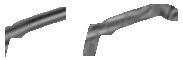
\includegraphics[width=0.7\linewidth]{terre5.jpg}
  \caption*{\textbf{Legenda:} \textit{``The Construction of new boundaries in the generated seismic images uses texture synthesis based on selected samples from the seismic image patches database.''}}
\end{figure}

\noindent\textbf{Citacao no manuscrito \texttt{(\_v7.tex, l.\,280)}:}
\begin{quoteblock}
\small
``[\ldots] Then, for each edge segment in the mask of the seismic texture image to be synthesized,
we synthesize its texture based on the patch with the most similar angle
\textbf{(see Fig.~5)}. We repeat this process until all the segments of the edge band are covered.''
\end{quoteblock}

\begin{checkblock}
\textbf{Checklist IEEE Access:}
\begin{itemize}[leftmargin=1.5em,topsep=2pt,itemsep=1pt]
  \item[$\square$] Resolucao $\geq$ 300 DPI (JPEG --- verificar compressao)
  \item[$\square$] Sem artefatos JPEG visiveis
  \item[$\square$] Considerar converter para PNG (sem perdas)
  \item[$\square$] Exportado diretamente do programa-fonte
  \item[$\square$] Cores funcionam em escala de cinza
\end{itemize}
\end{checkblock}

\noindent\textbf{Notas de revisao:}
\begin{mdframed}[linecolor=gray!30,backgroundcolor=white,innertopmargin=8pt,innerbottommargin=8pt]
  \vspace{3cm}
\end{mdframed}

\newpage

% ─── Figura 6 ────────────────────────────────────────────────────────────────
\figentry{6}{terre6.png}{fig:source1}{\colorbox{ok}{OK}}

\begin{figure}[h!]
  \centering
  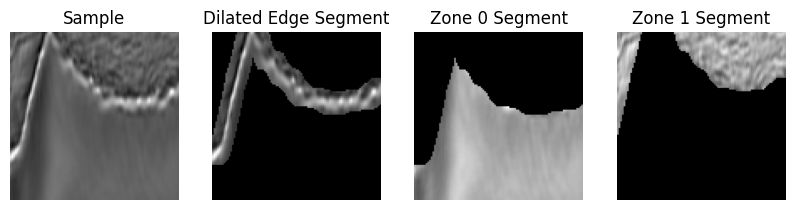
\includegraphics[width=0.7\linewidth]{terre6.png}
  \caption*{\textbf{Legenda:} \textit{``Real seismic saline images divided by context zones used as input to the texture synthesis process.''}}
\end{figure}

\noindent\textbf{Citacao no manuscrito \texttt{(\_v7.tex, l.\,296)}:}
\begin{quoteblock}
\small
``[\ldots] We divide the seismic image synthesis into steps to conform to the specific
characteristics of this kind of seismic image, such as the edge, saline rock, and conventional
rock zones, \textbf{as Fig.~6 shows}.''
\end{quoteblock}

\begin{checkblock}
\textbf{Checklist IEEE Access:}
\begin{itemize}[leftmargin=1.5em,topsep=2pt,itemsep=1pt]
  \item[$\square$] Resolucao $\geq$ 300 DPI
  \item[$\square$] Zonas de contexto claramente delimitadas e legiveis
  \item[$\square$] Sem fundo cinza / sem artefatos
  \item[$\square$] Exportado diretamente do programa-fonte
  \item[$\square$] Cores funcionam em escala de cinza
\end{itemize}
\end{checkblock}

\noindent\textbf{Notas de revisao:}
\begin{mdframed}[linecolor=gray!30,backgroundcolor=white,innertopmargin=8pt,innerbottommargin=8pt]
  \vspace{3cm}
\end{mdframed}

\newpage

% ─── Figura 9 ────────────────────────────────────────────────────────────────
\figentry{9}{terre9.png}{fig:synthetic\_samples}{\colorbox{ok}{OK}}

\begin{figure}[h!]
  \centering
  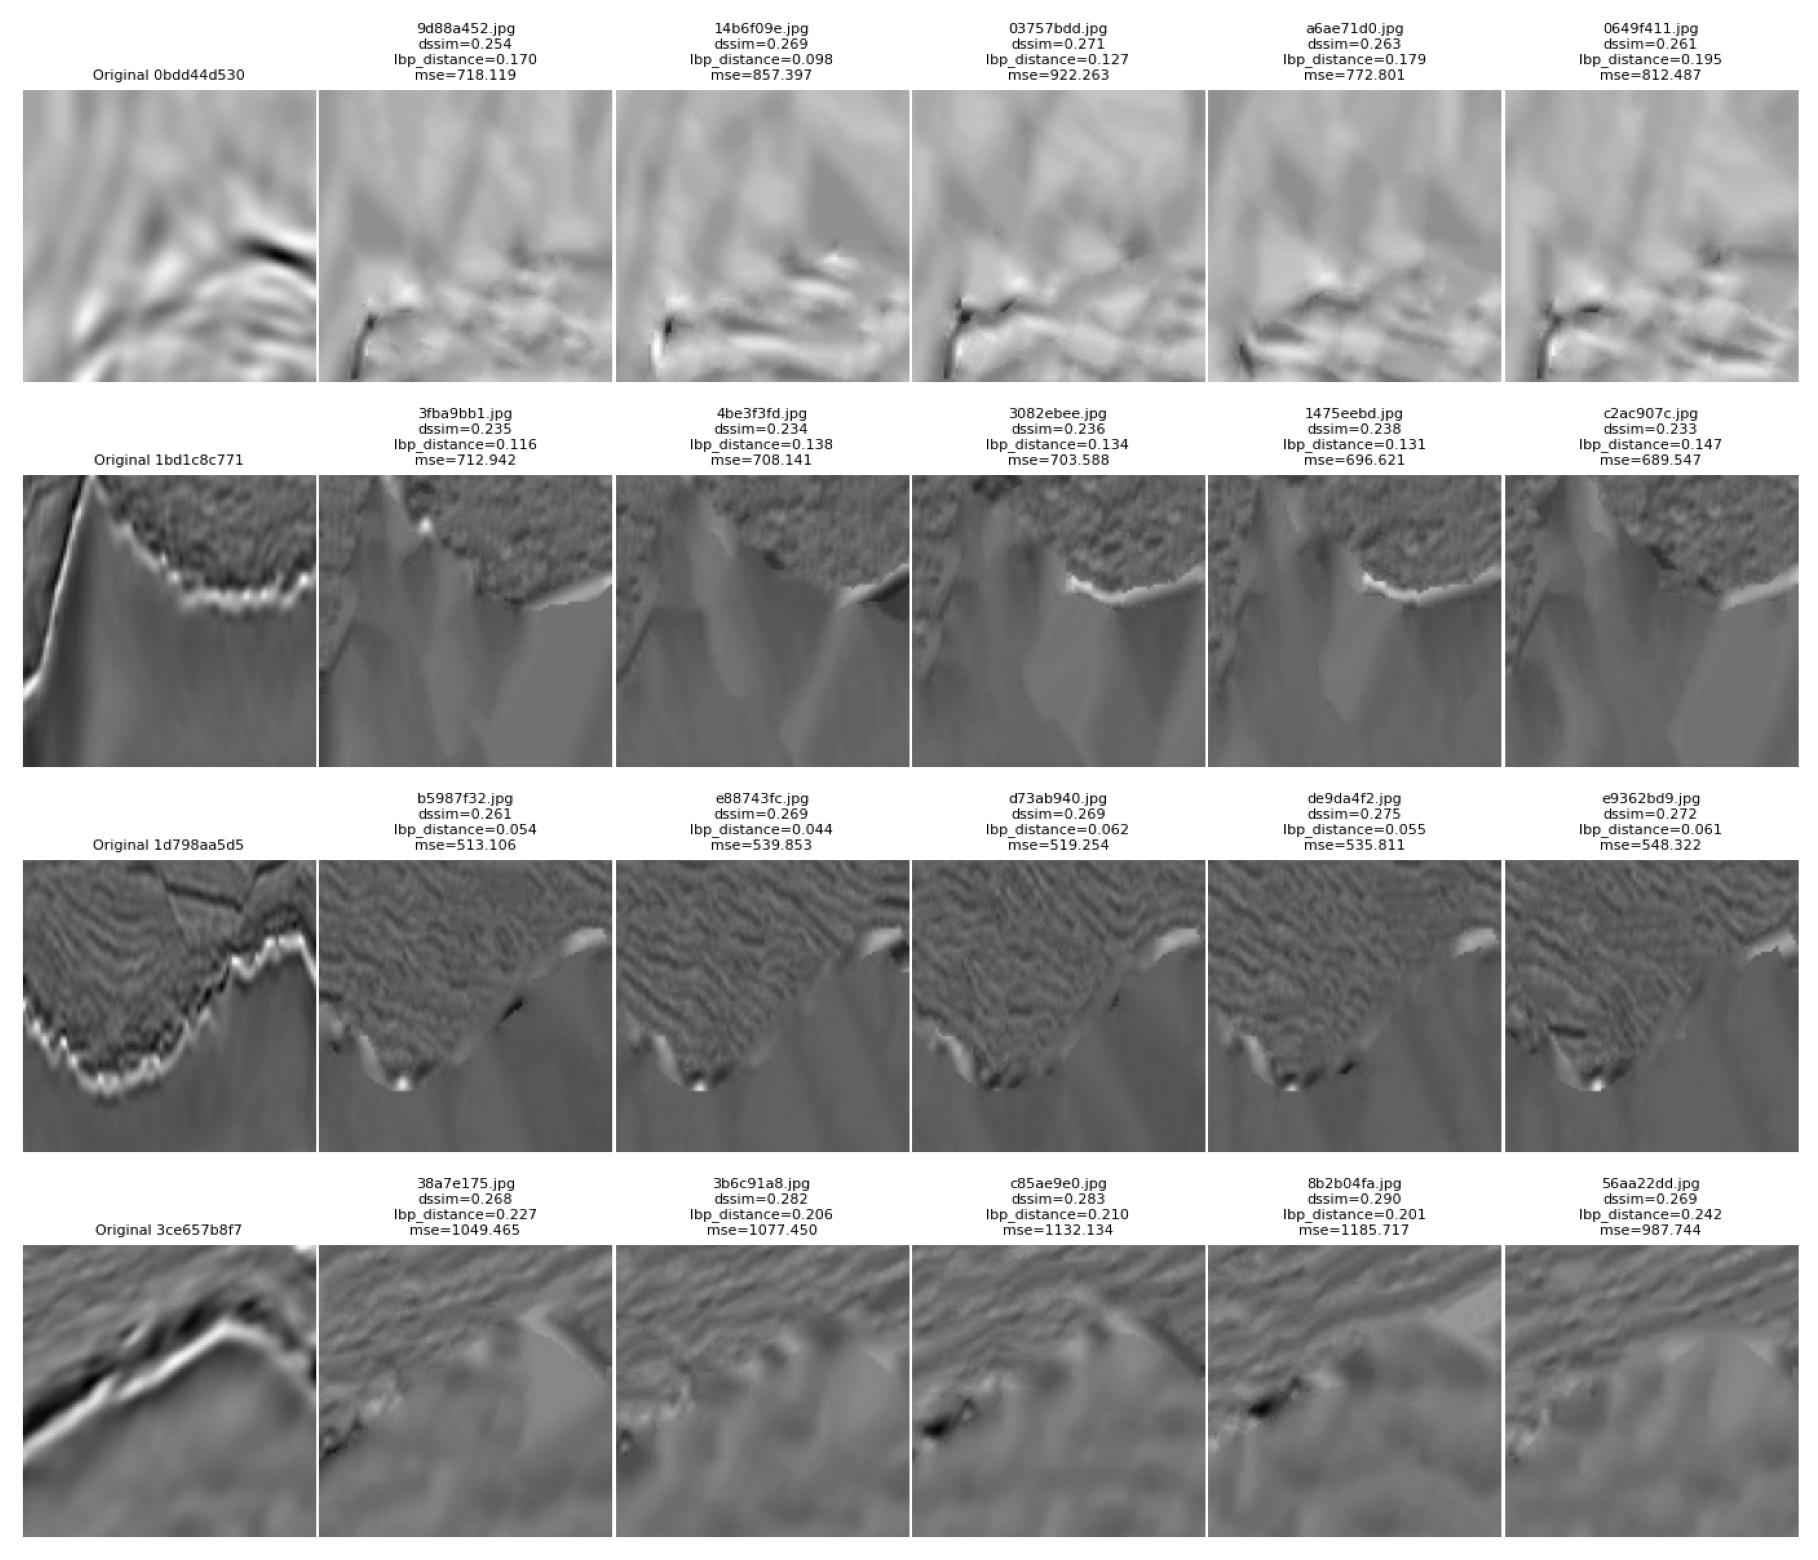
\includegraphics[width=0.7\linewidth]{terre9.png}
  \caption*{\textbf{Legenda:} \textit{``Synthetic Seismic Samples.''}}
\end{figure}

\noindent\textbf{Citacao no manuscrito \texttt{(\_v7.tex, l.\,401)}:}
\begin{quoteblock}
\small
``[\ldots] we evaluate the overlap between the experts selections of pixels corresponding to the
salt bodies in synthetic images and synthetic images masks,
\textbf{as illustrated in Fig.~9}.''
\end{quoteblock}

\begin{checkblock}
\textbf{Checklist IEEE Access:}
\begin{itemize}[leftmargin=1.5em,topsep=2pt,itemsep=1pt]
  \item[$\square$] Resolucao $\geq$ 300 DPI
  \item[$\square$] Sem fundo cinza / sem artefatos
  \item[$\square$] Amostras sinteticas visualmente representativas
  \item[$\square$] Exportado diretamente do programa-fonte
  \item[$\square$] Cores funcionam em escala de cinza
\end{itemize}
\end{checkblock}

\noindent\textbf{Notas de revisao:}
\begin{mdframed}[linecolor=gray!30,backgroundcolor=white,innertopmargin=8pt,innerbottommargin=8pt]
  \vspace{3cm}
\end{mdframed}

\newpage

% ─── Figura 10 ───────────────────────────────────────────────────────────────
\figentry{10}{terre10.png}{fig:expert2}{\colorbox{atencao}{ATENCAO --- verificar qualidade}}

\begin{figure}[h!]
  \centering
  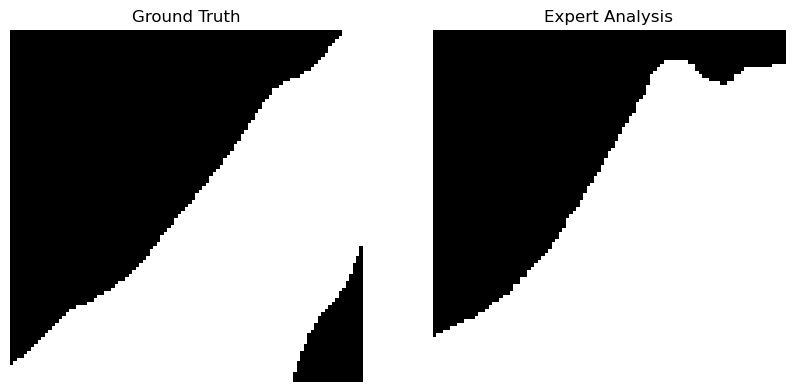
\includegraphics[width=0.7\linewidth]{terre10.png}
  \caption*{\textbf{Legenda:} \textit{``Quantitative analysis illustration using sample measurements for comparing the ground truth and expert analysis: Precision: 0.88; Recall: 0.87; F1-score: 0.87.''}}
\end{figure}

\noindent\textbf{Citacao no manuscrito \texttt{(\_v7.tex, l.\,401)}:}
\begin{quoteblock}
\small
``[\ldots] \textbf{Fig.~10 illustrates} the ground truth image and the specialist evaluation of the
salt bodies locations, and the computed precision, recall, and F1-score measures for this
particular case.''
\end{quoteblock}

\begin{checkblock}
\textbf{Checklist IEEE Access --- PRIORIDADE:}
\begin{itemize}[leftmargin=1.5em,topsep=2pt,itemsep=1pt]
  \item[$\square$] Resolucao $\geq$ 600 DPI (contem line art / texto)
  \item[$\square$] Exportado diretamente do programa-fonte (\textbf{NAO screenshot})
  \item[$\square$] Metricas (0.88 / 0.87) legiveis na impressao
  \item[$\square$] Sem fundo cinza
  \item[$\square$] Cores funcionam em escala de cinza
\end{itemize}
\end{checkblock}

\noindent\textbf{Notas de revisao:}
\begin{mdframed}[linecolor=gray!30,backgroundcolor=white,innertopmargin=8pt,innerbottommargin=8pt]
  \vspace{3cm}
\end{mdframed}

\newpage

% ════════════════════════════════════════════════════════════════════════════
\section*{Figuras Nao Referenciadas em \_v7.tex}
% ════════════════════════════════════════════════════════════════════════════

\begin{mdframed}[linecolor=orange!60,backgroundcolor=orange!5,roundcorner=4pt]
\textbf{Atencao:} As figuras abaixo existem na pasta \texttt{images/} mas \textbf{nao foram encontradas}
em nenhuma \texttt{\textbackslash{}includegraphics} do arquivo \texttt{\_v7.tex} atual.
Verifique se devem ser incluidas, substituidas ou removidas.
\end{mdframed}

\bigskip

% ─── terre7.png ──────────────────────────────────────────────────────────────
\subsection*{\texttt{terre7.png} --- Nao usada no \_v7.tex}

\noindent\textit{Nota: esta figura aparece em versoes anteriores do manuscrito
(\texttt{docs/Responses/r1c2-r2c5/\_v7.tex}).}

\begin{figure}[h!]
  \centering
  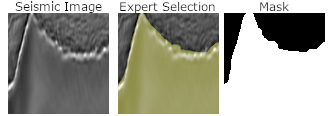
\includegraphics[width=0.55\linewidth]{terre7.png}
  \caption*{\textit{``Comparison between a real seismic image sample, and the geoscience specialist selection in terms of saline area and ground truth (saline mask).''}}
\end{figure}

\noindent\textbf{Decisao:}
\begin{mdframed}[linecolor=gray!30,backgroundcolor=white,innertopmargin=8pt,innerbottommargin=8pt]
  $\square$~Adicionar ao manuscrito \quad
  $\square$~Manter removida \quad
  $\square$~Substituir por outra versao\\[8pt]
  \vspace{1.5cm}
\end{mdframed}

\newpage

% ─── terre8.png ──────────────────────────────────────────────────────────────
\subsection*{\texttt{terre8.png} --- Nao referenciada}

\noindent\textit{Nenhuma referencia encontrada em nenhuma versao do manuscrito.
Verificar se e uma versao alternativa de outra figura ou pode ser excluida.}

\begin{figure}[h!]
  \centering
  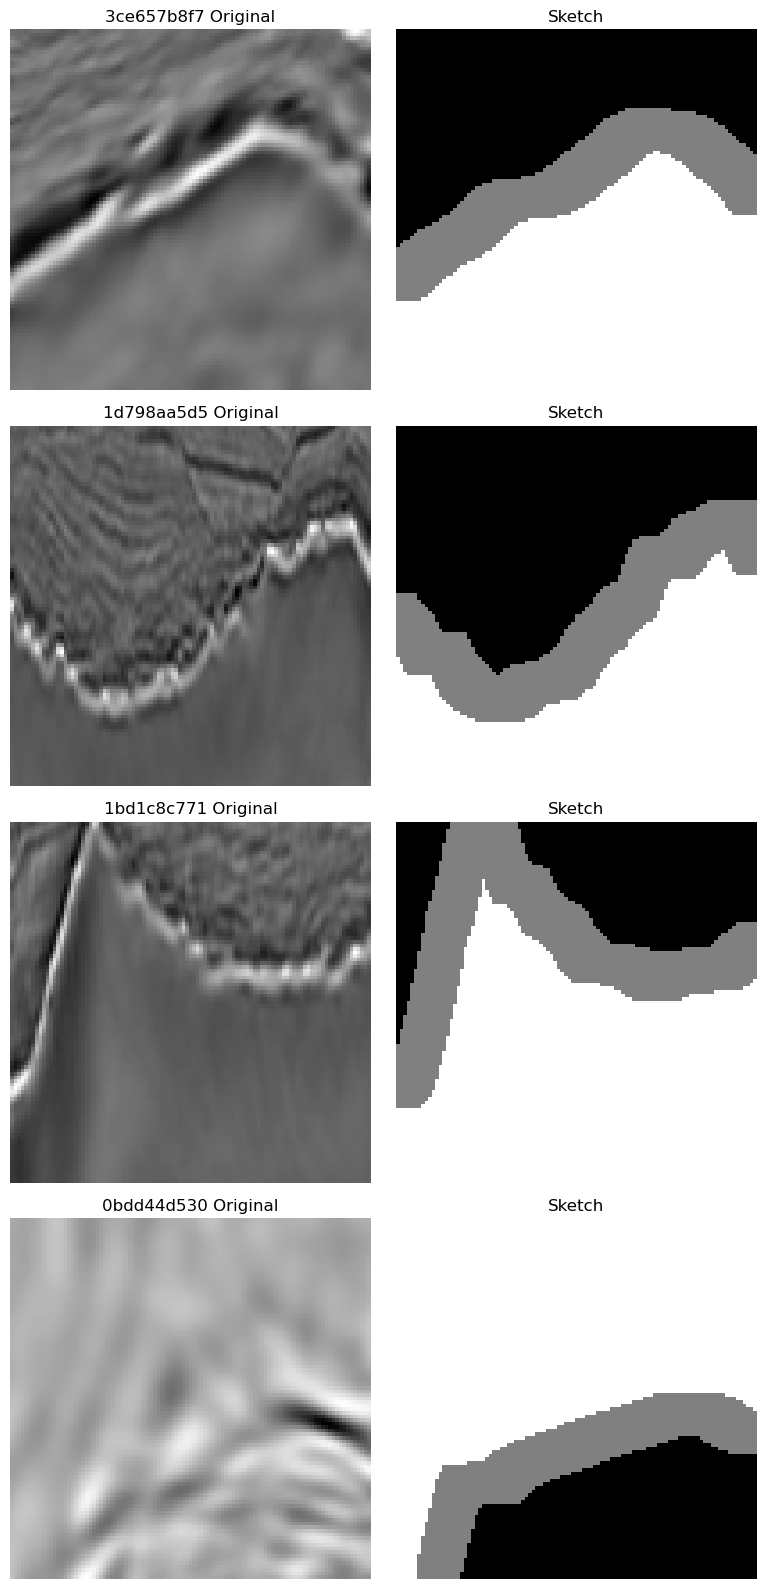
\includegraphics[width=0.55\linewidth]{terre8.png}
  \caption*{\textit{terre8.png --- sem referencia encontrada}}
\end{figure}

\noindent\textbf{Decisao:}
\begin{mdframed}[linecolor=gray!30,backgroundcolor=white,innertopmargin=8pt,innerbottommargin=8pt]
  $\square$~Adicionar ao manuscrito \quad
  $\square$~Excluir arquivo \quad
  $\square$~Arquivar em pasta separada\\[8pt]
  \vspace{1.5cm}
\end{mdframed}

\newpage

% ─── terre11.png ─────────────────────────────────────────────────────────────
\subsection*{\texttt{terre11.png} --- Nao referenciada}

\noindent\textit{Nenhuma referencia encontrada em nenhuma versao do manuscrito.
Verificar se e uma versao alternativa de outra figura ou pode ser excluida.}

\begin{figure}[h!]
  \centering
  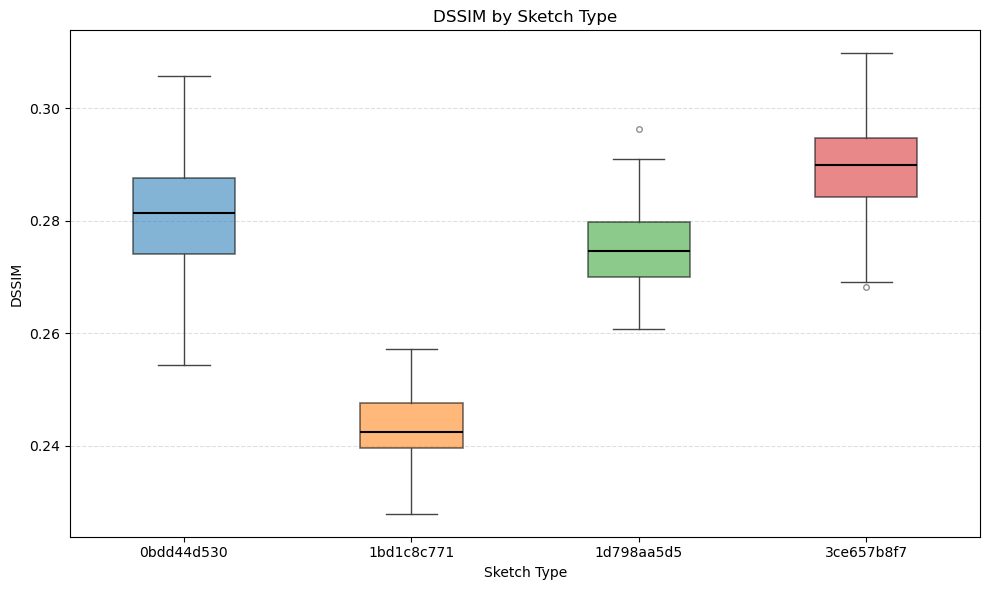
\includegraphics[width=0.55\linewidth]{terre11.png}
  \caption*{\textit{terre11.png --- sem referencia encontrada}}
\end{figure}

\noindent\textbf{Decisao:}
\begin{mdframed}[linecolor=gray!30,backgroundcolor=white,innertopmargin=8pt,innerbottommargin=8pt]
  $\square$~Adicionar ao manuscrito \quad
  $\square$~Excluir arquivo \quad
  $\square$~Arquivar em pasta separada\\[8pt]
  \vspace{1.5cm}
\end{mdframed}

\newpage

% ════════════════════════════════════════════════════════════════════════════
\section*{Fotos de Biografia}
% ════════════════════════════════════════════════════════════════════════════

\begin{minipage}[t]{0.48\textwidth}
  \subsection*{\texttt{terre.jpg} --- Luciano D.\ Terres}
  \begin{center}
    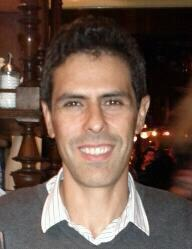
\includegraphics[width=1in,height=1.25in,clip,keepaspectratio]{terre.jpg}\\[4pt]
    {\small\textit{Foto de biografia --- Luciano}}
  \end{center}
  \begin{checkblock}
  \begin{itemize}[leftmargin=1.5em,topsep=2pt,itemsep=1pt]
    \item[$\square$] Dimensao: 1in $\times$ 1.25in
    \item[$\square$] Qualidade $\geq$ 300 DPI
    \item[$\square$] Fundo neutro
  \end{itemize}
  \end{checkblock}
\end{minipage}
\hfill
\begin{minipage}[t]{0.48\textwidth}
  \subsection*{\texttt{schar.jpg} --- Jacob Scharcanski}
  \begin{center}
    
\includegraphics[width=1in,height=1.25in,clip,keepaspectratio]{schar.jpg}\\[4pt]
    {\small\textit{Foto de biografia --- Jacob}}
  \end{center}
  \begin{checkblock}
  \begin{itemize}[leftmargin=1.5em,topsep=2pt,itemsep=1pt]
    \item[$\square$] Dimensao: 1in $\times$ 1.25in
    \item[$\square$] Qualidade $\geq$ 300 DPI
    \item[$\square$] Fundo neutro
  \end{itemize}
  \end{checkblock}
\end{minipage}

\newpage

% ════════════════════════════════════════════════════════════════════════════
\section*{Resumo de Acoes Necessarias}
% ════════════════════════════════════════════════════════════════════════════

\begin{table}[h!]
\centering
\renewcommand{\arraystretch}{1.5}
\begin{tabular}{clp{8cm}c}
\toprule
\textbf{Prioridade} & \textbf{Arquivo} & \textbf{Acao} & \textbf{Concluido?} \\
\midrule
\rowcolor{atencao} Alta  & terre10.png  & Verificar exportacao direta ($\geq$600 DPI); re-exportar se necessario & $\square$ \\
\rowcolor{atencao} Alta  & terre5.jpg   & Considerar conversao para PNG; verificar artefatos JPEG & $\square$ \\
\rowcolor{unused}  Media & terre7.png   & Decidir inclusao ou exclusao do \_v7.tex & $\square$ \\
\rowcolor{unused}  Media & terre8.png   & Verificar proposito; excluir ou arquivar & $\square$ \\
\rowcolor{unused}  Media & terre11.png  & Verificar proposito; excluir ou arquivar & $\square$ \\
\bottomrule
\end{tabular}
\end{table}

\bigskip
\noindent\textbf{Observacoes gerais:}
\begin{mdframed}[linecolor=gray!30,backgroundcolor=white,innertopmargin=8pt,innerbottommargin=8pt]
  \vspace{5cm}
\end{mdframed}

\end{document}
